\section{Required Background}
\begin{frame}[fragile]{Required Background} 
Set of Available Controllers:

\[action_1: \{ (\mathit{controller}_1^\mathit{action1}, \mathit{model}_1^\mathit{action1}), \dots \}\]
\[action_2: \{ (\mathit{controller}_1^\mathit{action2}, \mathit{model}_1^\mathit{action2}), \dots \}\]
\[\vdots\]
\[action_n:  \{ (\mathit{controller}_1^\mathit{actionN}, \mathit{model}_1^\mathit{actionN}), \dots \}\]
\end{frame}


\begin{frame}[fragile]{Required Background} 
\begin{block}{System Models}
\begin{enumerate}
  \item LTI drive model\pause
  \item LTI push model\pause
  \item Nonlinear push model
\end{enumerate}
\end{block}\pause

System Model Structure
  \[x(k+1) = f(x(k), u(k))\]
\end{frame}

\begin{frame}[fragile]{Required Background} 
\begin{block}{Control Methods}
\begin{enumerate}
  \item Model Predictive Control (MPC)
  \item Model Predictive Path Intergral (MPPI) control
\end{enumerate}
\end{block}
\end{frame}


\begin{frame}[fragile]{Required Background} 
\begin{block}{Driving}
\begin{enumerate}
  \item (MPC, \textit{lti-drive-model})
  \item (MPPI, \textit{lti-drive-model})
\end{enumerate}
\end{block}

\begin{block}{Pushing}
\begin{enumerate}
  \item (MPPI, \textit{lti-push-model})
  \item (MPPI, \textit{nonlinear-push-model})
\end{enumerate}
\end{block}
\end{frame}

\begin{frame}[fragile]{Required Background} 
  \begin{center}
    \hbox{\hspace{-1.5em} 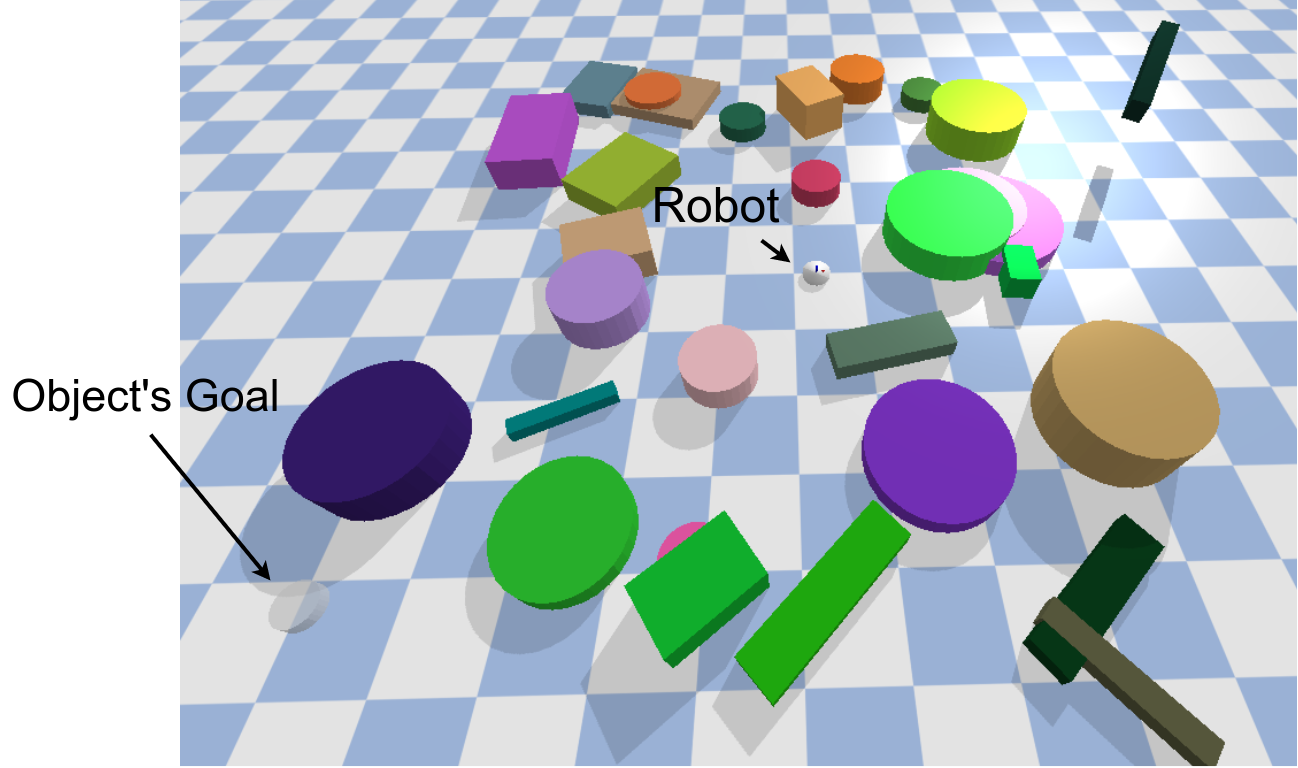
\includegraphics[height=0.85\textheight]{figures/required_background/is_there_a_path}}
  \end{center}
\end{frame}

\begin{frame}[fragile]{Required Background: Path Estimation} 
  \begin{center}
  \hbox{\hspace{0.0\textwidth} 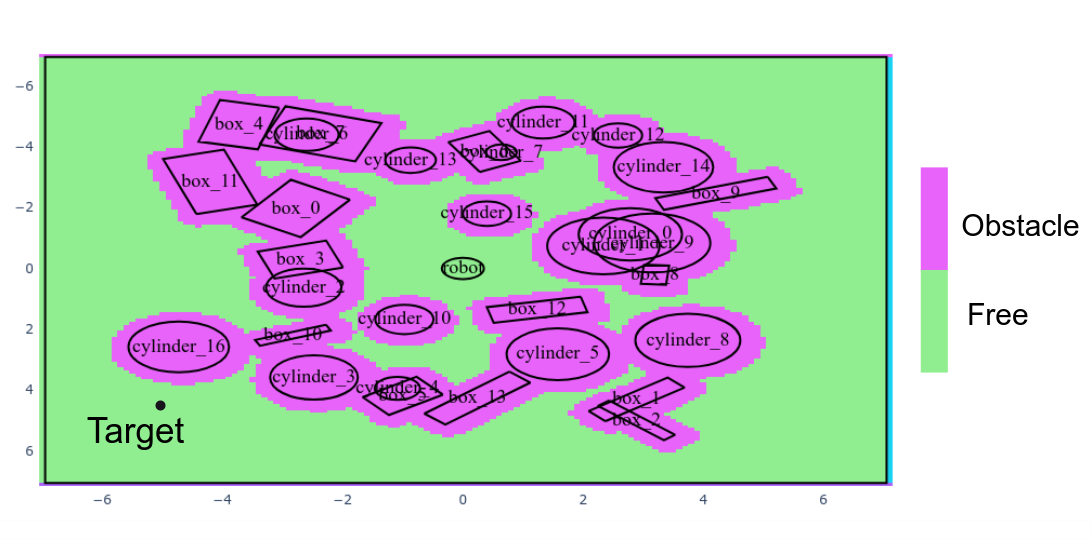
\includegraphics[width=1.0\textwidth]{figures/required_background/occupancy_grid} }
  \end{center}
\end{frame}

\begin{frame}[fragile]{Required Background: Path Planning} 
  \movie[width=\textwidth, height=0.3874\textwidth, autostart, poster]{}{figures/required_background/rrtvideo.mp4}
\end{frame}

\begin{frame}[fragile]{Required Background: Path Planning} 
  Double-tree Rapidly exploring Random Tree (RRT*) Algorithm~\cite{chen_fast_2018}:
  \begin{center}
  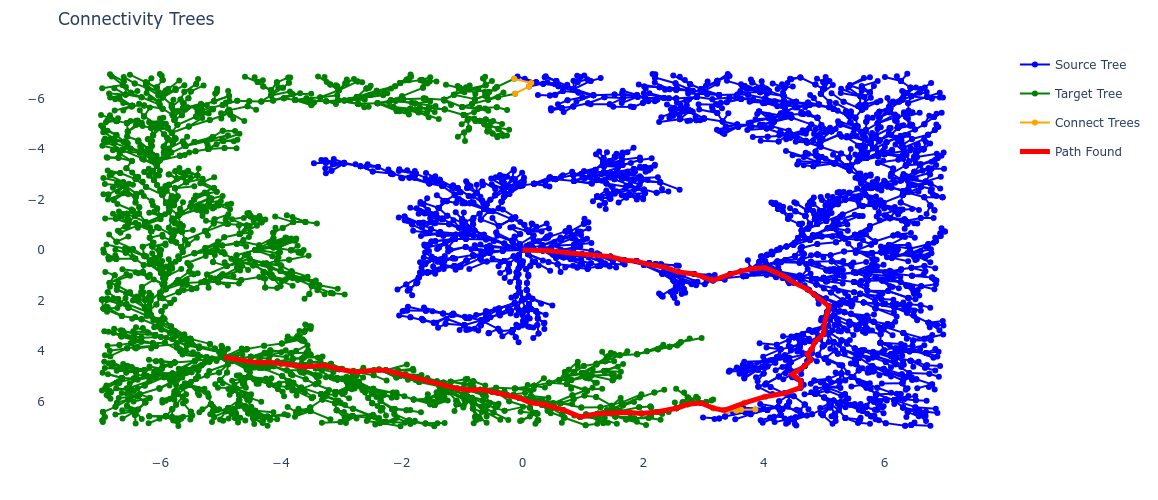
\includegraphics[width=0.8\textwidth]{figures/required_background/path_found}
  \end{center}
\[\mathit{Cost_{path}} = \sum_{i=1}^{n-1} \mathit{Distance}(c_i, c_{i+1})\]
\end{frame}
